\chapter{基于复杂网络理论的电网模型验证分析}
\label{cha:model}

\section{引言}
\label{sec:index2}
经典的电力网络分析是基于基尔霍夫电流电压方程、固定的拓扑结构来进行分析的。其研究已形成了较为完善的体系\cite{refs60}。随着科学技术的不断发展,电力系统
变得越来越复杂、规模越来越大。在网络拓扑和分析计算上,经典的电力网络分析方法因节点和线路复杂度高的问题上已不再适用。而从复杂网络角度来看,电力系统可以
简化成一个由节点(母线)和边(支路)构成的网络。在复杂网络理论的基础上进行电网结构研究分析,已成为电网结构脆弱性分析的发展趋势。

电力系统作为典型的复杂网络,在研究电力系统脆弱性之初,有必要对复杂网络的相关概念进行阐述和分析。本章首先阐述复杂网络的基本概念,在此基础上分析其基本特征
参数。此外,基于复杂网络的建模方法,分析验证复杂网络的两类模型,小世界模型和无标度模型。最后,在基本特征参数的基础上,分析与描述复杂网络的脆弱性,并研究
其脆弱性常用指标,为后续章节的电力系统结构脆弱性分析实验打下基础。

\section{复杂网络基本概念}
\label{sec:powersys}
复杂网络理论是把一个复杂系统抽象为网络,将复杂系统内的各个元件视为网络的节点,将元件之间的联系抽象为复杂网络中连接各个节点的边,由此建立起复杂网络模型。
复杂网络的基本概念主要包括复杂网络的概念描述和统计描述,概念描述主要包括复杂网络语言描述和特点及特性描述。统计描述主要包括网络的基本特征参数和静
态特性,研究复杂网络的基本概念对分析后续电力系统脆弱性指标有着重要的意义。

\subsection{复杂网络概念描述}
\label{sec:composite}
复杂网络这一概念,人们试图严格去定义复杂系统,但直到现在还未充分认识和了解复杂网络,故难以给出其严格和实用的定义\cite{refs61}。目前普遍认同的是,钱学森
院士等人发起研究的系统科学研究领域——开放的复杂巨系统理论中对复杂网络的定义:具有自组织、自相似、吸引子、小世界、无标度中部分或全部性质的网络称为复杂网络
\footnote{摘自中文维基百科}。下面其性质进行具体阐述:

$(1)$自组织:对于这一概念,从不同学科角度来看会有不同的解读,我们从系统论的观点来看,“自组织”是指一个系统在内在机制的驱动下,自行从简单到复杂、从粗糙
向细致方向发展。不断提高自身的复杂度和精细度的过程。其与“他组织”的区别在于:“他组织”是靠外部指令而形成的组织,而“自组织”是系统按照内在机制自动形成的有序结构。
一个系统自组织属性愈强,其保持和产生新功能的能力也愈强。

$(2)$自相似:是指复杂网络的总体与部分、这一部分与另一部分之间的精细结构或性质所具有的相似性,或者可以这样理解:从整体中取出局部(局域)能够体现整体的基
本特征。

$(3)$吸引子:是微积分和系统科学论中的概念。一个系统有朝某个稳态发展的趋势,这个稳态叫做吸引子。吸引子是一个数学概念,描述系统运动的收敛类型,它存在于相平面。
简言之,吸引子是一个集合,当时间趋向于无穷大时,在任何一个有界集上出发的非定常流的所有轨迹都趋向于这个集合。

$(4)$小世界性:网络的小世界性是指对具有较短平均路径又具有较高聚类系数的网络性质的一种定义。平均路径长度和聚类系数会在下一小节展开描述。

$(5)$无标度性:网络的无标度性是指对网络的度分布符合幂律分布的复杂网络性质的一种定义。具体来讲,复杂网络只有少数节点拥有大量的连接,而大部分节点却很少。

% 在以上系统科学的角度理解的基础上,给出以下对复杂网络比较直观的特性论述:

%$(1)$开放性

%复杂系统是开放的,受外界影响,复杂系统及其子系统与系统的环境之间有物质、能量和信息的交换。

%$(2)$复杂性

%复杂系统中的子网络的种类繁多,子网络之间存在多种形式、多种层次的交互作用。

%$(3)$进化涌现性

%在特定条件下,系统中各元件或各子系统之间相互作用。在此期间会有微小变化,但系统能自组织、自加强、自协调,并随之扩大、发展,发生质变。这种质变,在复杂系统中称为
%涌现。


\subsection{复杂网络统计描述}
\label{sec:feature}
在刻画复杂网络结构的统计特性上提出了许多概念和特征参数,其中包含四个基本的特征参数:度及度分布、平均路径长度、聚类系数和介数及介数分布。一般一个无权无向的抽象网络用
$\boldsymbol{M}=(\boldsymbol{V}, \boldsymbol{E})$表示,$\boldsymbol{V}$为节点集合,$\boldsymbol{E}$为边集合。

$(1)$节点度及度分布:

节点$v_i$的度$k_i$定义为与该节点连接的所有节点的数量。直观来讲,一个节点的度越大,这个节点在某种情况下越重要。

网络的度分布可用分布函数$P(k)$来描述,$P(k)$的定义为网络中度为$k$的节点数量在整个网络中所占的比例,换言之,网络中节点度为$k$的概率为$P(k)$

$(2)$平均路径长度:

将网络中两个节点$v_i$和$v_j$之间的距离$d_{ij}$定义为连接这两个节点的最短路径上的边数,$L$定义为所有节点对之间最短距离的均值。

\begin{equation}
    \label{equ:chap3:feature}
    L=\frac{1}{C_N^2} \sum_{i \neq j} d_{i j}
\end{equation}

式中:$N$为网络节点数。

$(3)$聚类系数:

聚类系数是一个表征两个节点间连接紧密程度的特征参数。当节点$v_i$的节点度为$k_i$,那么相邻节点之间的边数最大为$\frac{k_i(k_i-1)}{2}$,假设节点$v_i$的$k_i$和邻居节点
之间实际存在的边数为$E_i$,那么节点$v_i$的聚类系数定义为:$C_i=\frac{2E_i}{k_i(k_i-1)}$。网络的聚类系数为:

\begin{equation} 
    \label{equ:chap3:feature}
    C=\frac{1}{N} \sum_{i=1}^N C_i
\end{equation}

式中:$N$为网络节点数。

$(4)$介数及介数分布

网络中的不相邻节点$v_i$和$v_j$之间的最短路径会途经某些节点或边,如果某些节点$v$或边$e$被其他许多最短路径经过,则表示该节点对网络的贡献较大,重要性也越高。将节点介数
$B(v)$和边介数$B(e)$分别定义为:

\begin{equation} 
    \label{equ:chap3:feature}
    B(v)=\sum_{i \neq j\in V} \frac{\sigma_{ij}(v)}{\sigma_{ij}} 
\end{equation}
\begin{equation} 
    \label{equ:chap3:feature}
    B(e)=\sum_{i \neq j\in V} \frac{\sigma_{ij}(e)}{\sigma_{ij}} 
\end{equation}

式中:$\sigma_ij$是节点$v_i$和$v_j$间最短路径的数量,$\sigma_ij(v)$是节点$v_i$和$v_j$通过节点v的最短路径数量,$\sigma_ij(e)$是节点$v_i$和$v_j$通过支路e的最短路
径数量。

\section{基于复杂网络理论的电网模型性质分析}
\label{sec:wind}

\subsection{小世界模型}
\label{sec:windEffects}
在复杂网络理论中,将现实中的复杂网络抽象成节点和边,比如人脉、互联网和电网。Watts和Strogatz将这类具有高聚集程度、小平均距离的网络称为小世界网络\cite{refsWS}。提出小世界模型
(WS模型)。其构造过程为:首先构造一个最近邻连接的规则网络,然后以概率$p$随机断开网络上的一条边后重新连接边。当$p$为0时,网络为规则网络,当$p$为1时,网络为随机网络。当$0<p<1$
时,网络为小世界网络。当重连概率$p$介于0—1变化时,网络模型的聚类系数和平均距离也在发生变化,其演变过程如图\ref{fig:SW}所示。
\begin{figure}[H] % use float package if you want it here
    \centering
    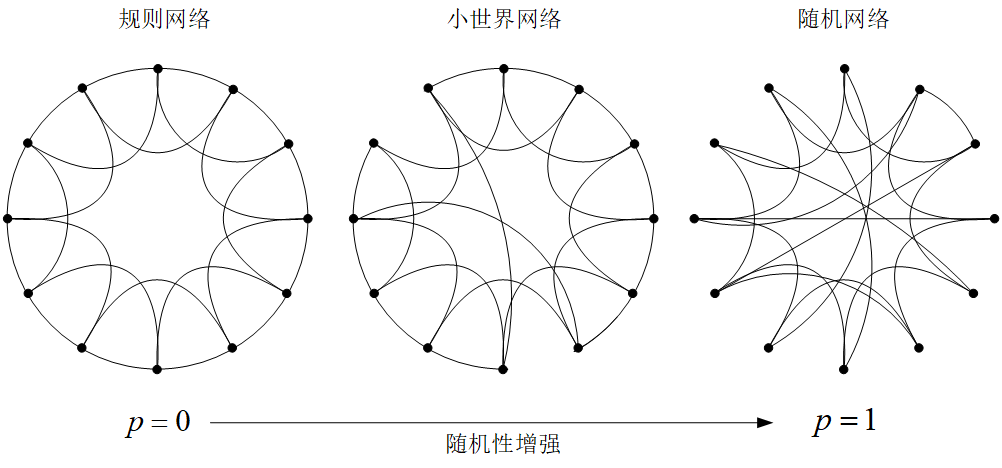
\includegraphics[width=14cm,height=6.5cm]{SW_network.png}
    \caption{小世界网络模型示意图}
    \label{fig:SW}
  \end{figure}




\subsection{无标度模型}
\label{sec:windModel}



\section{复杂网络的脆弱性描述}
\label{sec:load}



\subsection{脆弱性概念}
\label{sec:loadEffect}




\subsection{脆弱性常用指标}
\label{sec:loadModel}




\section{本章小结}
\label{sec:sum2}





